
A continuous surface $S$ in $\reals^3$ is called {\em $xy$-monotone} if
every line parallel to the $z$-axis intersects it at a single point
at most. For example, the sphere $x^2 + y^2 + z^2 = 1$ is {\em not}
$xy$-monotone as the $z$-axis intersects it at $(0, 0, -1)$ and at
$(0, 0, 1)$; however, if we use the $xy$-plane to split it to an
upper hemisphere and a lower hemisphere, these two hemispheres are
$xy$-monotone.

An $xy$-monotone surface can therefore be represented as a
bivariate function $z = S(x,y)$, defined over some continuous range
$R_S \subseteq \reals^2$. Given a set $\calS = \{ S_1, S_2, \ldots,
S_n \}$ of $xy$-monotone surfaces, their {\em lower envelope} is defined
as the point-wise minimum of all surfaces. Namely, the lower envelope
of the set $\calS$ can be defined as the following function:
\begin{eqnarray*}
\calL_{\calS} (x,y) = \min_{1 \leq k \leq n}{
\begin{ccTexOnly}\overline{S}\end{ccTexOnly}
\begin{ccHtmlOnly}<span style="text-decoration:overline">S</span>\end{ccHtmlOnly}
_k (x,y)} \ ,
\end{eqnarray*}
where we define $
\begin{ccTexOnly}\overline{S}\end{ccTexOnly}
\begin{ccHtmlOnly}<span style="text-decoration:overline">S</span>\end{ccHtmlOnly}
_k(x,y) = S_k(x,y)$ for $(x,y) \in R_{S_k}$, and $
\begin{ccTexOnly}\overline{S}\end{ccTexOnly}
\begin{ccHtmlOnly}<span style="text-decoration:overline">S</span>\end{ccHtmlOnly}
_k(x,y) = \infty$ otherwise.

Similarly, the {\em upper envelope} of $\calS$ is the point-wise maximum of
the $xy$-monotone surfaces in the set:
\begin{eqnarray*}
\calU_{\calS} (x,y) = \max_{1 \leq k \leq n}{
\begin{ccTexOnly}\underline{S}\end{ccTexOnly}
\begin{ccHtmlOnly}<span style="text-decoration:underline">S</span>\end{ccHtmlOnly}
_k (x,y)} \ ,
\end{eqnarray*}
where in this case $
\begin{ccTexOnly}\underline{S}\end{ccTexOnly}
\begin{ccHtmlOnly}<span style="text-decoration:underline">S</span>\end{ccHtmlOnly}
_k(x,y) = -\infty$ for $(x,y) \not\in
R_{S_k}$.

Given a set of $xy$-monotone surfaces $\calS$, the {\em minimization
diagram} of $\calS$ is a subdivision of the $xy$-plane into cells,
such that the identity of the surfaces that induce the lower diagram
over a specific cell of the subdivision (be it a face, an edge or
a vertex) is the same. In non-degenerate situation, a face is
induced by a single surface (or by no surfaces at all, if there are
no $xy$-monotone surfaces defined over it), and an edge is induced
by a single surface and corresponds to its projected boundary, or by
two surfaces and corresponds to their projected intersection curve.
The {\em maximization diagram} is symmetrically defined for upper envelopes.
In the rest of this chapter, we refer to both these diagrams as
{\em envelope diagrams}.

It is easy to see that an envelope diagram is no more than a planar
arrangement (see Chapter~\ref{chapterArrangement_2}), represented
using an extended \dcel\ structure, such that every \dcel\ record
(namely each face, halfedge and vertex) stores an additional container
of it originators: the $xy$-monotone surfaces that induce this feature.

Lower and upper envelopes can be efficiently computed using a
divide-and-conquer approach. First note that the envelope diagram for
a single $xy$-monotone curve $S_k$ is trivial to compute: we project
the boundary of its range of definition $R_{S_k}$ onto the $xy$-plane
and label the faces it induces accordingly. Given a set $\hat{\calS}$
of (non necessarily $xy$-monotone) surfaces in $\reals^3$, we start by
subdividing each surface into a finite number of weakly $xy$-monotone
surfaces\footnote{To handle degenerate inputs, we consider {\em vertical}
surfaces, namely patches of planes that are perpendicular to the
$xy$-plane, as {\em weakly} $xy$-monotone.}, obtaining the set $\calS$.
We continue by splitting the set into two disjoint subsets $\calS_1$
and $\calS_2$, and we compute their envelope diagrams recursively.
We finally have to merge the diagrams, and we do this by overlaying
them and then applying some post-processing on the resulting diagram.
The post-processing stage is non-trivial and involves the projection
of intersection curves onto the $xy$-plane --- 
see~\cite{cgal:m-rgece-06} for more details.

\section{The Envelope-Traits Concept}
%====================================

In order to make the envelope-computation algorithm generic and
handle arbitrary surfaces, it is parameterized with a traits class,
which defines the geometry of surfaces it handles and supports all
the necessary functionality one these surfaces and on their 
projections onto the $xy$-plane. The traits class must be a model
of the \ccc{EnvelopeTraits_3} concept, whose details are given in
this section.

As the representation of envelope diagrams is based on 2D
arrangements, and the envelop-computation algorithm employs overlay
of planar arrangements, the \ccc{EnvelopeTraits_3} refines the
\ccc{ArrangementXMonotoneTraits_2} concept. Namely, a model of this concept
must define the planar types \ccc{Point_2} and \ccc{X_monotone_curve_2}
and support basic operations on them, as listed
in Section~\ref{arr_sec:traits}. Moreover, it must define the spacial
types \ccc{Surface_3} and \ccc{Xy_monotone_surface_3} (in practice,
these two types may be the same). Any model of the envelope-traits
concept must also support the following operations on these spacial
types:

\begin{figure}[t]
\begin{ccTexOnly}
  \begin{center}
  \begin{tabular}{ccc}
    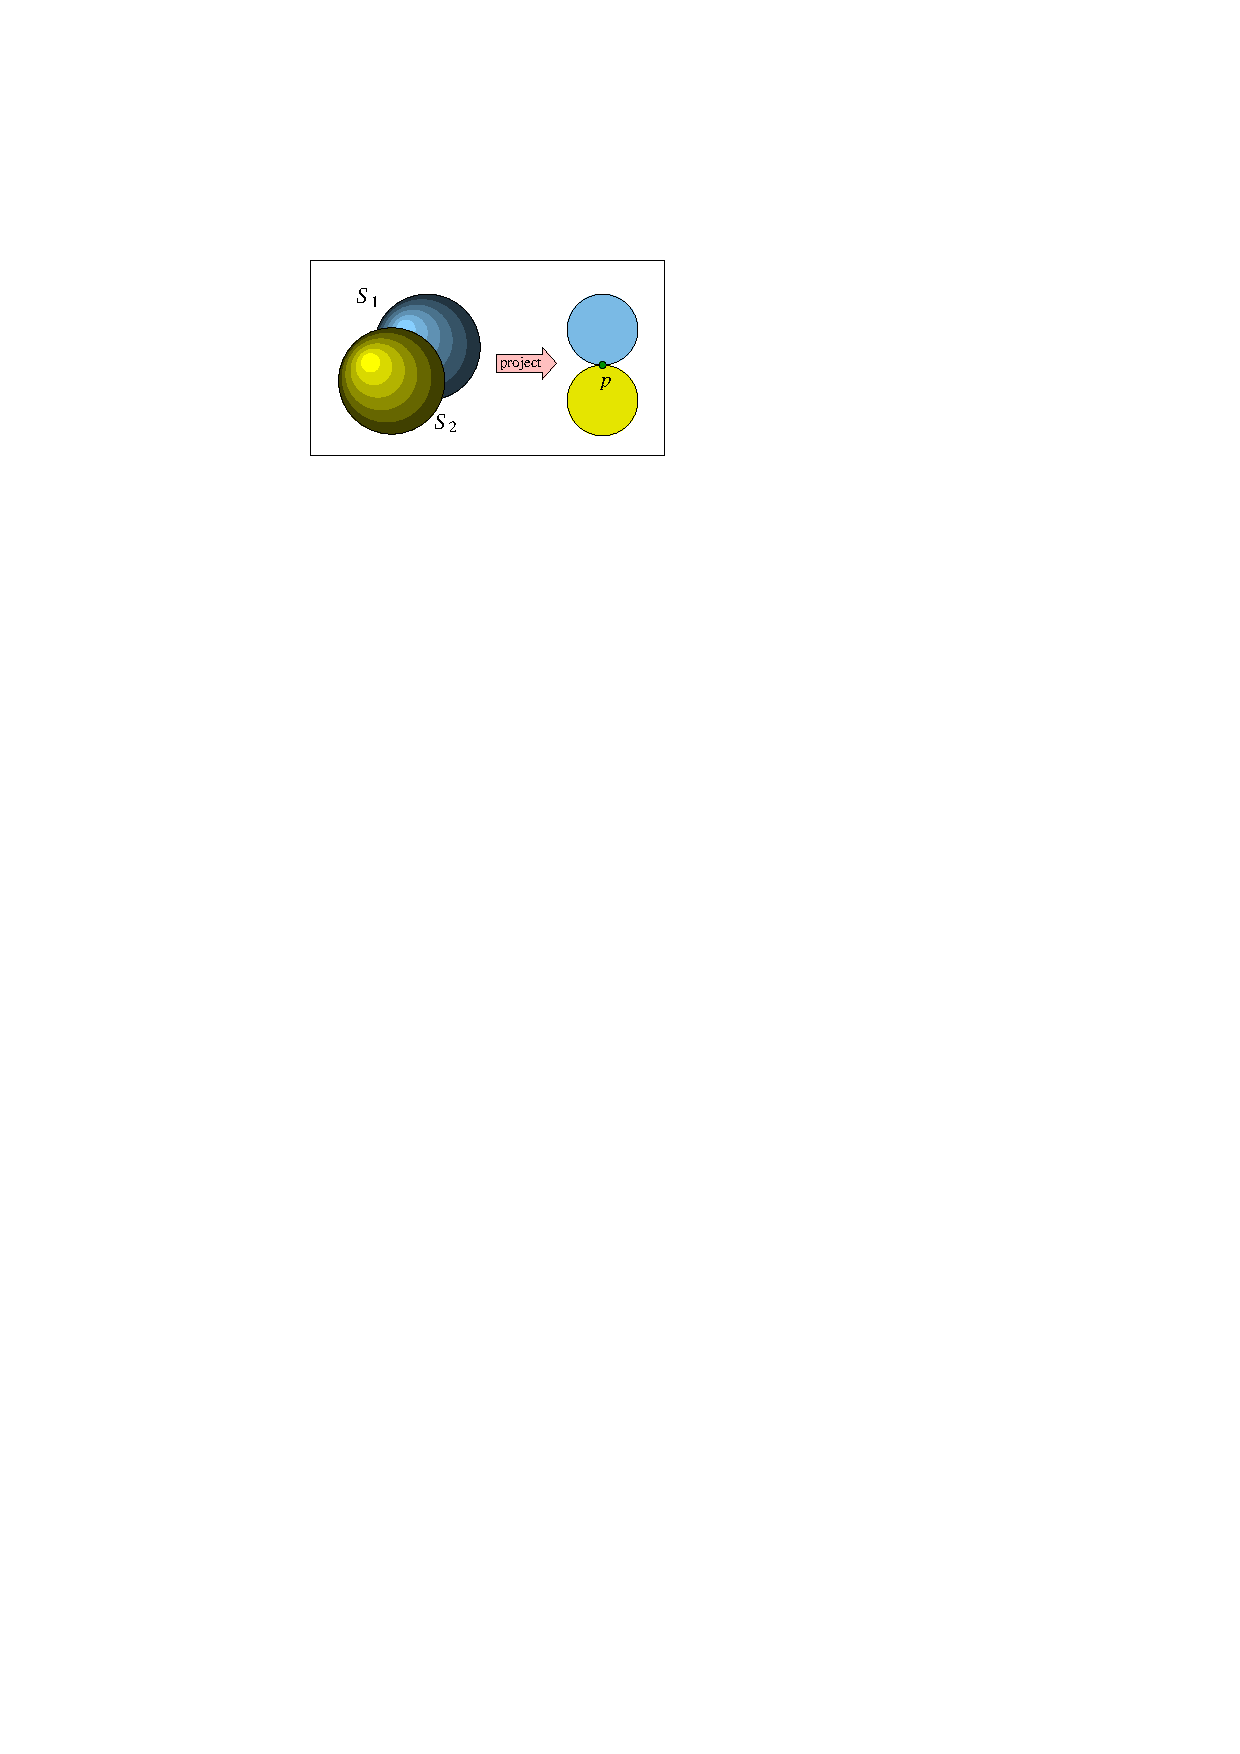
\includegraphics{Envelope_3/fig/compare_over_point} & ~ &
    
\includegraphics{Envelope_3/fig/compare_over_curve} \\
    {\small (a)} & ~ & {\small (b)}
  \end{tabular}
  \end{center}
\end{ccTexOnly}
\begin{ccHtmlOnly}
  <p><center>
  <table>
  <tr>
  <td><img src="./fig/compare_over_point.gif" border=0 alt="Traits-class operations."></td>
  <td><img src="./fig/compare_over_curve.gif" border=0 alt="Traits-class operations."></td>
  </tr>
  <tr align="center"><td>(a)</td><td>(b)</td></tr>
  </table>
  </center>
\end{ccHtmlOnly}
\caption{(a) The spheres $S_1$ and $S_2$ have only one
two-dimensional point $p$ in their common $xy$-definition range. They
do not necessarilyintersect over this point, and the
envelope-construction algorithm needs to determine their relative
$z$-order over $p$. (b) The $z$-order of the surfaces $S_1$ and $S_2$
should be determined over the $x$-monotone curve $c$. The comparison
is performed over the {\em interior} of $c$, excluding its
endpoints.\label{env3_fig:comp_over}}
\end{figure}

\begin{itemize}
\item Subdivide a given surface into continuous $xy$-monotone
surfaces. It is possible to disregard $xy$-monotone surfaces
that do not contribute to the surface envelope at this stage
(for example, if we are given a sphere, it is possible to return
just its lower hemisphere if we are interested in the lower
envelope; the upper hemisphere is obviously redundant).
%
\item Given an $xy$-monotone surface $S$, construct all planar
curves that form the boundary of the vertical projection $S$'s
boundary onto the $xy$-plane.

This operation is used at the bottom of the recursion to build the
minimization diagram of a single $xy$-monotone surface.
%
\item Construct all geometric entities that comprise the projection
(onto the $xy$-plane) of the intersection between two $xy$-monotone
surfaces $S_1$ and $S_2$. These entities may be:
  \begin{itemize}
  \item A planar curve, which is the projection of an 3D intersection
  curve of $S_1$ and $S_2$ (for example, the intersection curve
  between two spheres is a 3D circle, which becomes an ellipse when
  projected onto the $xy$-plane).
  %
  In many cases it is also possible to indicate the multiplicity of
  the intersection: if it is odd, the two surfaces intersect
  transversely and change their relative $z$-positions on either
  side of the intersection curve; if it the multiplicity is even,
  they maintain their relative $z$-position.
  Providing the multiplicity information is optional. When provided,
  it is used by the algorithm to determine the relative order of $S_1$
  and $S_2$ on one side of their intersection curve when their order
  on the other side of that curve is known, thus improving the
  performance of the algorithm.
  \item A point, induces by the projection of a tangency point
  of $S_1$ and $S_2$, {\em or} by the projection of a vertical
  intersection curve onto the $xy$-plane.
  \end{itemize}
Needless to say, the set of intersection entities may be empty in
case $S_1$ and $S_2$ do not intersect.
%
\item Given two $xy$-monotone surfaces $S_1$ and $S_2$, and a
planar point $p = (x_0,y_0)$ that lies in their common $xy$-definition
range, determine the $z$-order of $S_1$ and $S_2$ over $p$,
namely compare $S_1(x_0,y_0)$ and $S_2(x_0,y_0)$.
%
This operation is used only in degenerate situations, in order to
determine the surface inducing the envelope over a vertex (see
Figure~\ref{env3_fig:comp_over}(a) for an illustration of a situation
when this operation is used).
%
\item Given two $xy$-monotone surfaces $S_1$ and $S_2$, and a
planar $x$-monotone curve $c$, which is a part of their projected
intersection, determine the $z$-order of $S_1$ and $S_2$ immediately
above (or, similarly, immediately below) the curve $c$. Note that $c$
is a planar $x$-monotone curve, and we refer to the region above
(or below) it in the {\it plane}. If $c$ is a vertical curve, we regard
the region to its left as lying above it, and the region to its right
as lying below it.

This operation is used by the algorithm to determine the surface that
induce the envelope over a face incident to $c$.
%
\item Given two $xy$-monotone surfaces $S_1$ and $S_2$, and a
planar $x$-monotone curve $c$, which fully lies in their common
$xy$-definition range, and such that $S_1$ and $S_2$ do not intersect
over the interior of $c$, determine the relative $z$-order of $s_1$
and $s_2$ over the interior of $c$. Namely, we compare $S_1(x_0,y_0)$
and $S_2(x_0,y_0)$ for some point $(x_0, y_0)$ on $c$.

This operation is used by the algorithm to determine which surface
induce the envelope over an edge associated with the $x$-monotone
curve $c$, or of a face incident to $c$, in situations where the
previous predicate cannot be used, as $c$ is {\em not} an intersection
curve of $S_1$ and $S_2$ (see Figure~\ref{env3_fig:comp_over}(b) for
an illustration of a situation where this operation is used).
\end{itemize}

The package currently contains a traits class for named
\ccc{Env_triangle_traits_3<Kenrel>} handling 3D triangles, and another
named \ccc{Env_sphere_traits_3<ConicTraits>} for 3D spheres, based
on geometric operations on conic curves (ellipses). In addition, the
package includes a traits-class decorator that enables users to attach
external (non-geometric) data to surfaces. The usage of the various
traits classes is demonstrated in the next section.

\section{Examples}
%=================

\begin{figure}[t]
\begin{ccTexOnly}
  \begin{center}
  \begin{tabular}{ccc}
    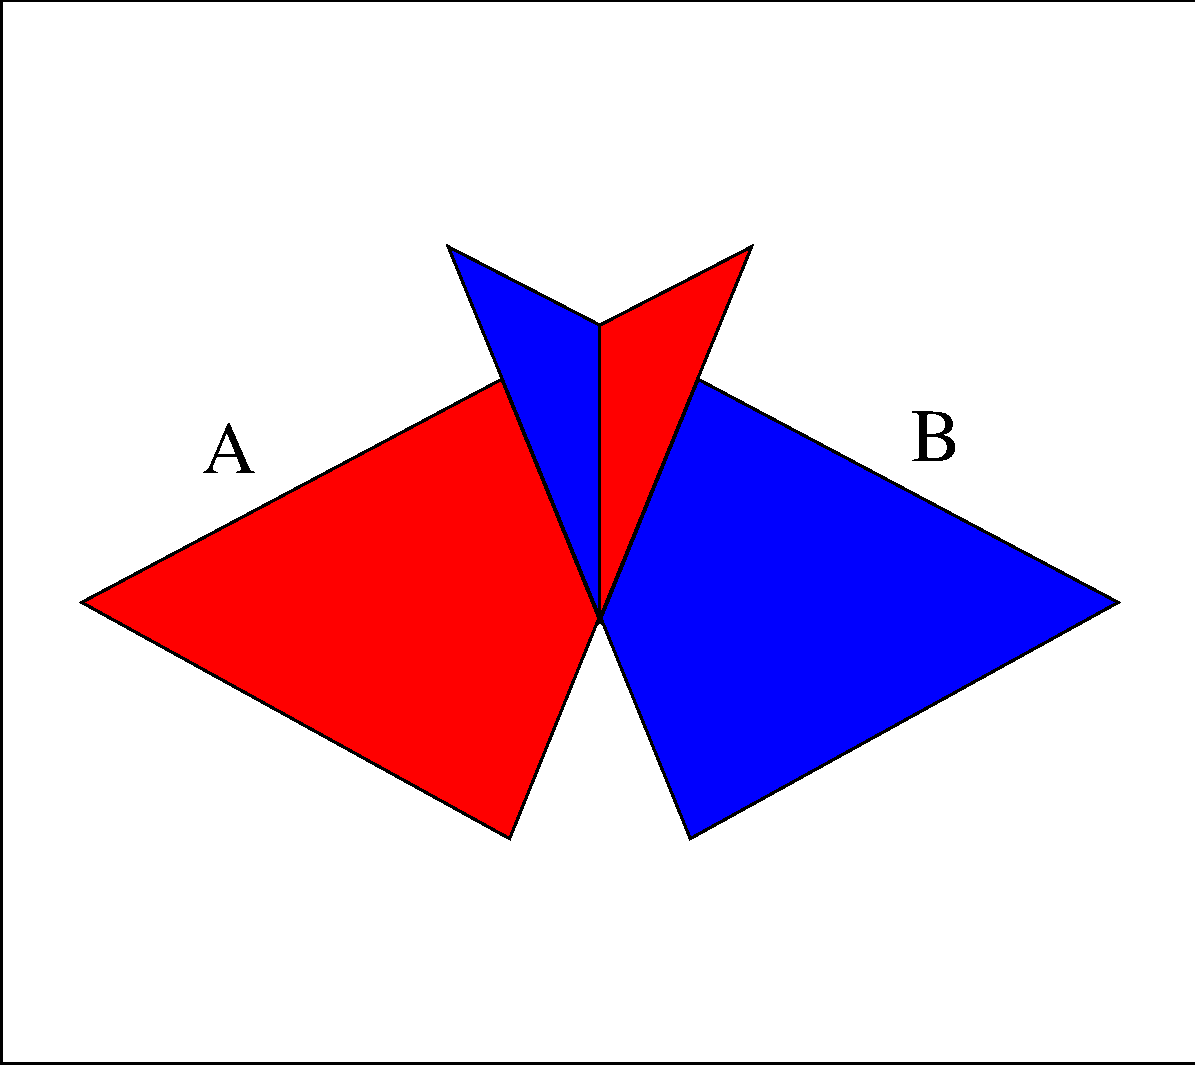
\includegraphics[height=1.8in]{Envelope_3/fig/ex_triangles} &
    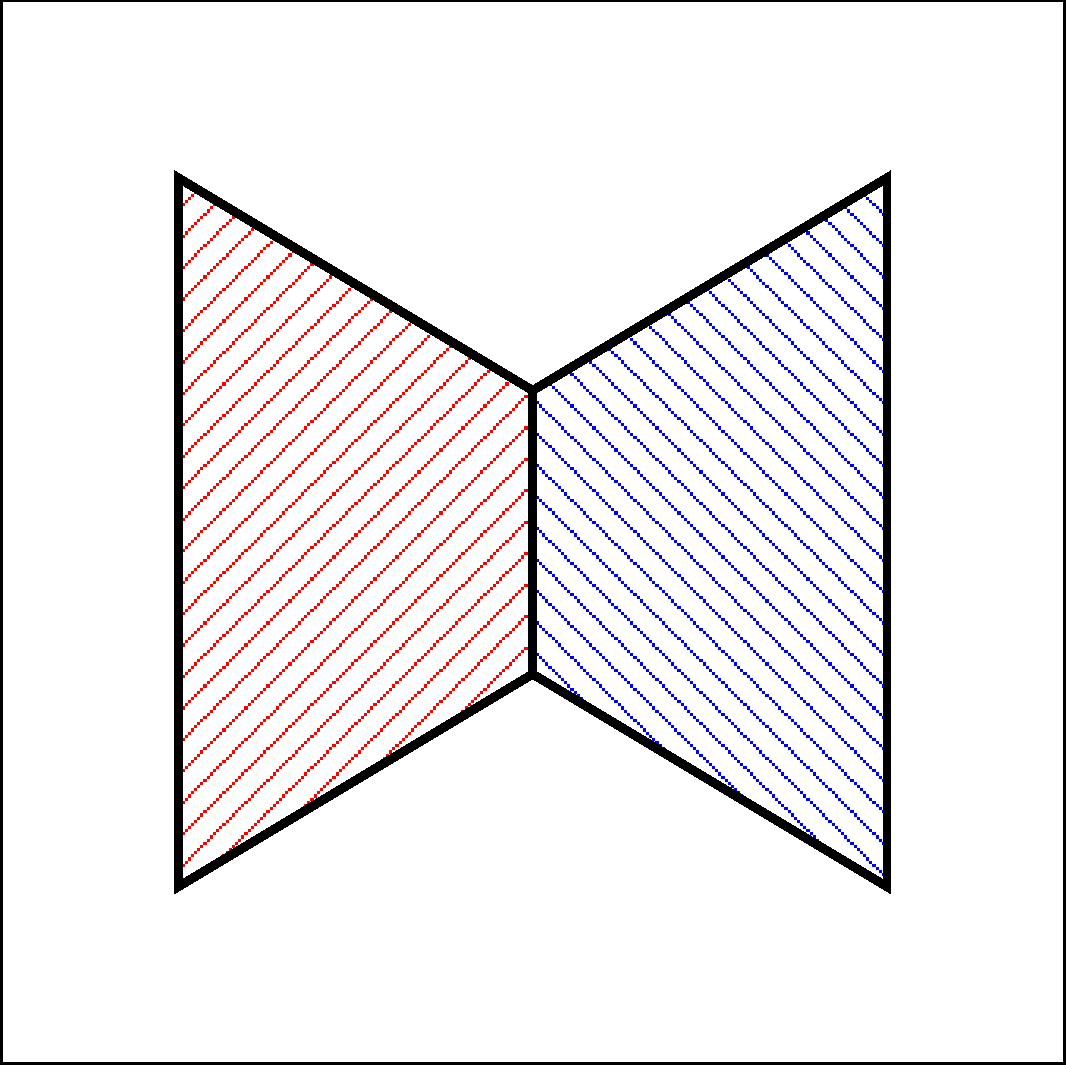
\includegraphics[height=1.8in]{Envelope_3/fig/ex_tri_le} &
    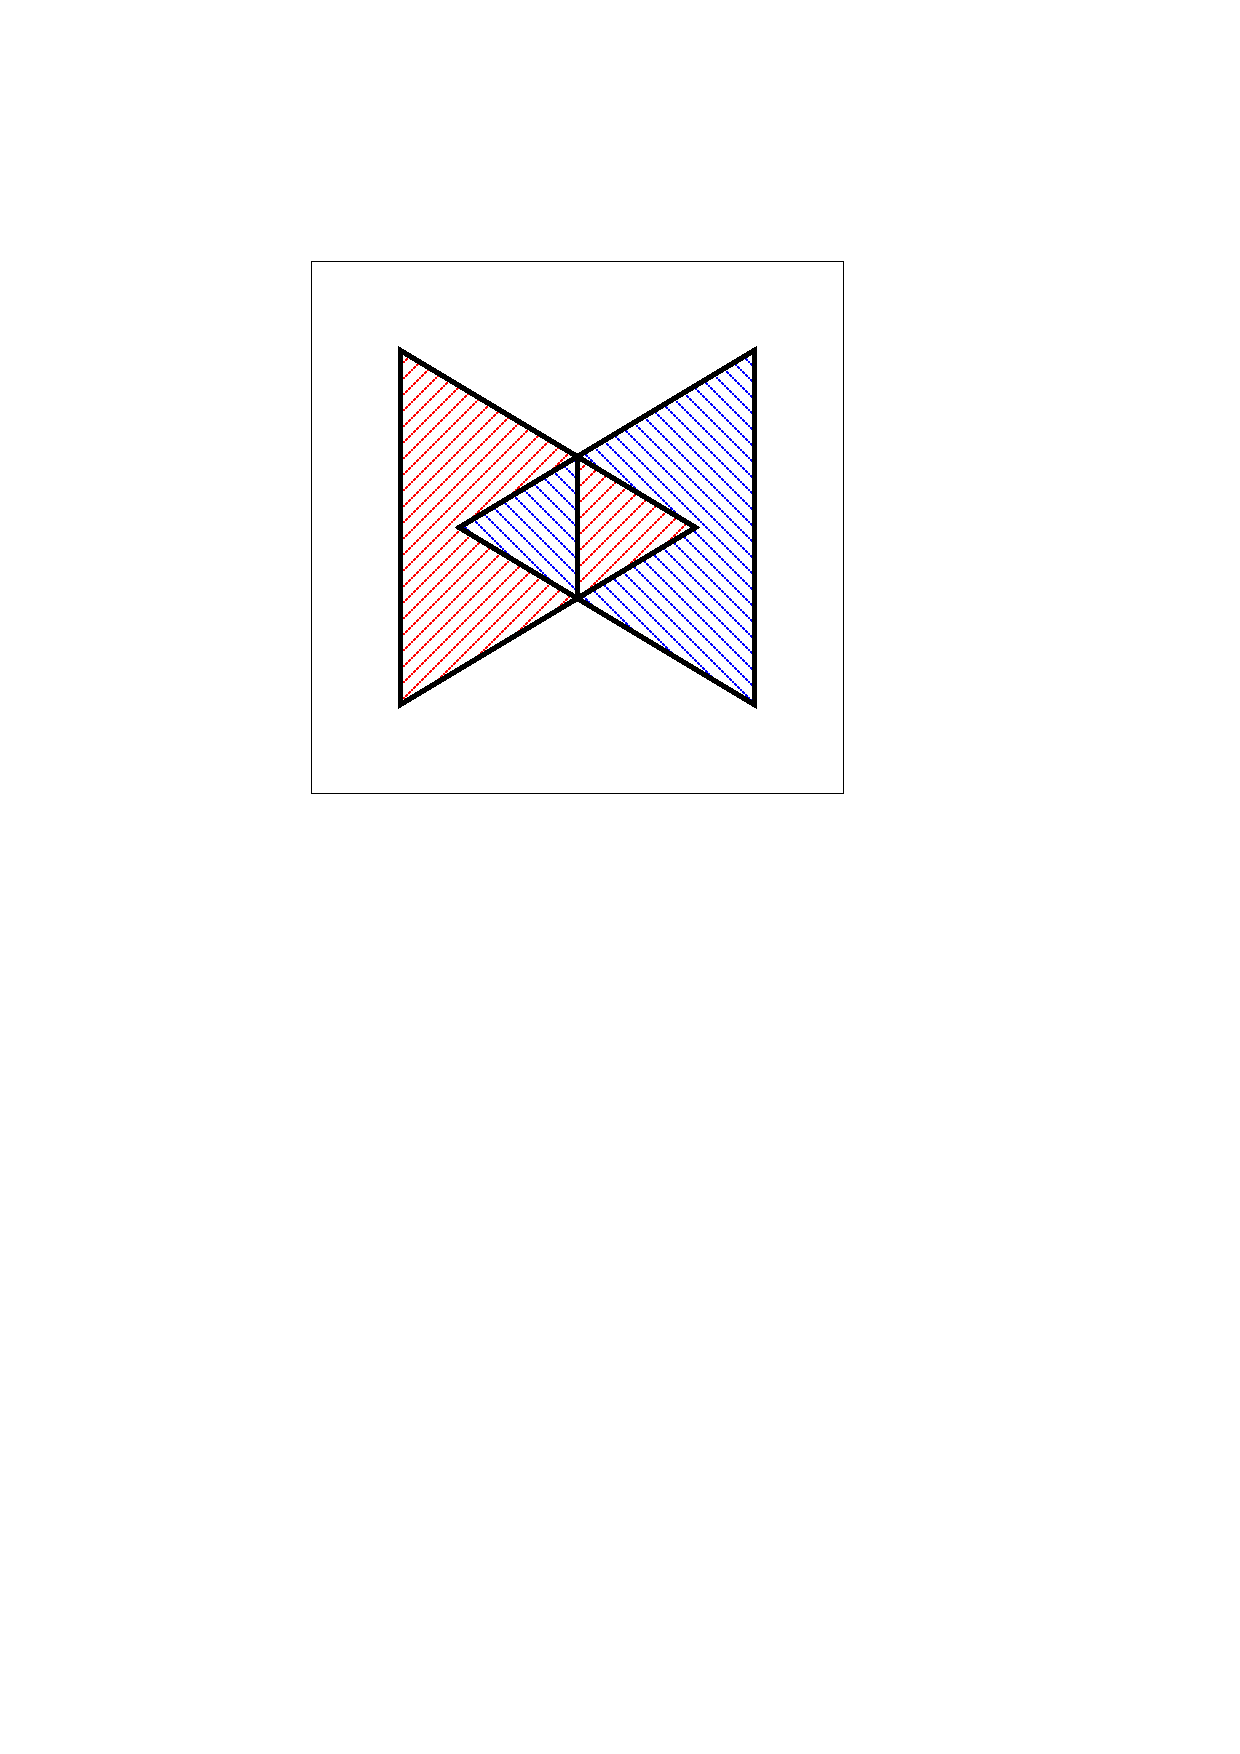
\includegraphics[height=1.8in]{Envelope_3/fig/ex_tri_ue} \\
    {\small (a)} & {\small (b)} & {\small (c)}
  \end{tabular}
  \end{center}
\end{ccTexOnly}
\begin{ccHtmlOnly}
  <p><center>
  <table>
  <tr>
  <td><img src="./fig/ex_triangles.gif" border=0 alt="ex_triangles"></td>
  <td><img src="./fig/ex_tri_le.gif" border=0 alt="ex_tri_le"></td>
  <td><img src="./fig/ex_tri_ue.gif" border=0 alt="ex_tri_ue"></td>
  </tr>
  <tr align="center"><td>(a)</td><td>(b)</td><td>(c)</td></tr>
  </table>
  </center>
\end{ccHtmlOnly}
\caption{(a)~Two triangles in $\reals^3$, as given in
\ccc{ex_envelope_triangles.cpp}. (b)~Their lower envelope.
(c)~Their upper envelope.\label{env3_fig:ex_tri}}
\end{figure}

The following example shows how to use the envelope-traits class
for 3D triangles and how to traverse the envelope diagram. It
constructs the lower and upper envelopes of the two triangles,
as depicted in Figure~\ref{env3_fig:ex_tri}(a) and prints the
triangles that induce each face and each edge in the output diagrams.
For convenience, we use the traits-class decorator
\ccc{Env_surface_data_traits_3} to label the triangles. When
printing the diagrams, we just output the labels of the triangles:

\ccIncludeExampleCode{Envelope_3/ex_envelope_triangles.cpp}

The next example demonstrates how to instantiate and use the
envelope-traits class for spheres, based on the
\ccc{Arr_conic_traits_2} class that handles the projected intersecion
curves. The program reads a set of spheres from an input file and
constructs their lower envelope:

\ccIncludeExampleCode{Envelope_3/ex_envelope_spheres.cpp}
